\documentclass[12pt, letterpaper]{article}
\usepackage[utf8]{inputenc}
\usepackage[T1]{fontenc}
\usepackage[document]{ragged2e}
\usepackage{amsmath}
\usepackage{fullpage}
\usepackage{color}
\usepackage[table]{xcolor}
\usepackage{listings}
\usepackage{graphicx}

\lstset{
  aboveskip=3mm,
  belowskip=-2mm,
  backgroundcolor=\color{white},
  basicstyle=\footnotesize,
  breakatwhitespace=false,
  breaklines=true,
  captionpos=b,
  commentstyle=\color{red},
  deletekeywords={...},
  escapeinside={\%*}{*)},
  extendedchars=true,
  framexleftmargin=16pt,
  framextopmargin=3pt,
  framexbottommargin=6pt,
  frame=tb,
  keepspaces=true,
  keywordstyle=\color{blue},
  language=scilab,
  literate=
  {á}{{\'a}}1 {é}{{\'e}}1 {í}{{\'i}}1 {ó}{{\'o}}1 {ú}{{\'u}}1
  {Á}{{\'A}}1 {É}{{\'E}}1 {Í}{{\'I}}1 {Ó}{{\'O}}1 {Ú}{{\'U}}1
  {à}{{\`a}}1 {è}{{\`e}}1 {ì}{{\`i}}1 {ò}{{\`o}}1 {ù}{{\`u}}1
  {À}{{\`A}}1 {È}{{\'E}}1 {Ì}{{\`I}}1 {Ò}{{\`O}}1 {Ù}{{\`U}}1
  {ä}{{\"a}}1 {ë}{{\"e}}1 {ï}{{\"i}}1 {ö}{{\"o}}1 {ü}{{\"u}}1
  {Ä}{{\"A}}1 {Ë}{{\"E}}1 {Ï}{{\"I}}1 {Ö}{{\"O}}1 {Ü}{{\"U}}1
  {â}{{\^a}}1 {ê}{{\^e}}1 {î}{{\^i}}1 {ô}{{\^o}}1 {û}{{\^u}}1
  {Â}{{\^A}}1 {Ê}{{\^E}}1 {Î}{{\^I}}1 {Ô}{{\^O}}1 {Û}{{\^U}}1
  {œ}{{\oe}}1 {Œ}{{\OE}}1 {æ}{{\ae}}1 {Æ}{{\AE}}1 {ß}{{\ss}}1
  {ű}{{\H{u}}}1 {Ű}{{\H{U}}}1 {ő}{{\H{o}}}1 {Ő}{{\H{O}}}1
  {ç}{{\c c}}1 {Ç}{{\c C}}1 {ø}{{\o}}1 {å}{{\r a}}1 {Å}{{\r A}}1
  {€}{{\EUR}}1 {£}{{\pounds}}1,
  morekeywords={*,...},
  numbers=left,
  numbersep=10pt,
  numberstyle=\tiny\color{black},
  rulecolor=\color{black},
  showspaces=false,
  showstringspaces=false,
  showtabs=false,
  stepnumber=1,
  stringstyle=\color{gray},
  tabsize=4,
  title=\lstname,
}

\title{TD Calcul Numérique}
\author{BOUTON Nicolas}

\pagenumbering{gobble}

\begin{document}

\maketitle

Information : Les codes se trouvent à la fin du pdf (page 28).

\newpage

\section*{Exercice 1}

\begin{enumerate}
\item Voir la fonction \textbf{pointgauche} dans le fichier
  "exo1.sci".

  \underline{Calcul :}

  \begin{equation*}
    I \approx h \sum_{i = 0}^{n-1}{f(a + ih)}
  \end{equation*}


  \underline{Explication du code :}
  \begin{itemize}
    \item Le code est trivial et bien commenté.
  \end{itemize}
  
  \underline{Résultat numérique :} \newline
  Pour l'appel de fonction suivant : \newline
  \textbf{res = pointgauche(0, 10, mysquare, 100);} \newline
  où :
  \begin{itemize}
  \item \textbf{0} correspond au début de l'intervale
  \item \textbf{10} correspond à la fin de l'intervale
  \item \textbf{mysquare} correspond à la fonction $x^2$ qui se trouve
    dans \newline "myfunc.sci"
  \item \textbf{100} correspond au nombre de pas
  \end{itemize}

  On obtient : \textbf{res = 328.35}
  
\item Voir la fonction \textbf{trapeze} dans le fichier "exo1.sci".

  \underline{Calcul :}

  \begin{equation*}
    I \approx h \left( \frac{1}{2} f(a) + \sum_{i = 1}^{n-1}{f(a + ih)} + \frac{1}{2} f(b) \right)
  \end{equation*}

  \underline{Explication du code :}
  \begin{itemize}
    \item Le code est trivial et bien commenté.
  \end{itemize}
  
  \underline{Résultat numérique :} \newline
  Pour l'appel de fonction suivant : \newline
  \textbf{res = trapeze(0, 10, mysquare, 100);} \newline
  où :
  \begin{itemize}
  \item \textbf{0} correspond au début de l'intervale
  \item \textbf{10} correspond à la fin de l'intervale
  \item \textbf{mysquare} correspond à la fonction $x^2$ qui se trouve
    dans \newline "myfunc.sci"
  \item \textbf{100} correspond au nombre de pas
  \end{itemize}

  On obtient : \textbf{res = 333.35}

\item Voir la fonction \textbf{int\_simpson} dans le fichier
  "exo1.sci".

  \underline{Calcul :}

  \begin{equation*}
    \begin{split}
      I \approx & \frac{h}{6} \left[ f(a) + 2 \left( \sum_{i = 1}^{n - 1}
        {f(a + ih)} \right) + f(b) \right. \\
        + & \left. 4 \left( \sum_{i = 0}^{n - 1} {f \left(a + \left(i +
        \frac{1}{2} \right)h \right) } \right)
        \right]
    \end{split}
  \end{equation*}

  \underline{Explication du code :}
  \begin{itemize}
  \item La boucle contenant \textbf{somme\_a\_ih} calcul la somme :
    \begin{equation*}
      \sum_{i = 1}^{n - 1} f(a + ih)
    \end{equation*}
  \item La boucle contenant \textbf{somme\_a\_i2h} calcul la somme :
    \begin{equation*}
      \sum_{i = 0}^{n - 1} f(a + (i + \frac{1}{2})h)
    \end{equation*}
  \end{itemize}
  
  \underline{Résultat numérique :} \newline
  Pour l'appel de fonction suivant : \newline
  \textbf{res = int\_simpson(0, 10, mysquare, 100);} \newline
  où :
  \begin{itemize}
  \item \textbf{0} correspond au début de l'intervale
  \item \textbf{10} correspond à la fin de l'intervale
  \item \textbf{mysquare} correspond à la fonction $x^2$ qui se trouve
    dans \newline "myfunc.sci"
  \item \textbf{100} correspond au nombre de pas
  \end{itemize}

  On obtient : \textbf{res = 333.33333}


\item Voir la fonction \textbf{sin\_pi\_x} dans le fichier
  "exo1.sci".\newline 

  Sur l'intervale $[0, 1]$ et un nombre de pas de 10  on obtient :
  \begin{itemize}
  \item $ 0.6313752 $ pour \textbf{pointgauche}
  \item $ 0.6313752 $ pour \textbf{trapeze}
  \item $ 0.6366219 $ pour \textbf{int\_simpson}
  \end{itemize}

  On voit que \textbf{pointgauche} et \textbf{trapeze} ont la même
  approximation, cela peut s'expliquer par leurs taux de convergences
  qui est le même.\newline

  Maintenant si on prend un nombre de pas de 20 on obtient :
    \begin{itemize}
    \item $ 0.6353102 $ pour \textbf{pointgauche}
    \item $ 0.6353102 $ pour \textbf{trapeze}
    \item $ 0.6366119 $ pour \textbf{int\_simpson}
    \end{itemize}

    Si on compare l'écart des résultat on obtient :
    \begin{itemize}
    \item $ 0.0040550 $ pour \textbf{pointgauche}
    \item $ 0.0040550 $ pour \textbf{trapeze}
    \item $ 0.00001 $ pour \textbf{int\_simpson}
    \end{itemize}

    On voit que l'erreur relative de \textbf{pointgauche} et \textbf{trapeze}
    est plus grand que \textbf{int\_simpson}, ce qui confirme leurs
    taux de convergence plus bas que \textbf{int\_simpson}.
        
\end{enumerate}

\section*{Exercice 2}

On a le système suivant :

$$
\left\{
\begin{array}{l}
  p(-3) = 3 \\
  p(-1) = 7 \\
  p(3) = 7 \\
  p(5) = -3
\end{array}
\right.
$$

Utilisons la métode des \textbf{différence divisé} :

\textit{Premiére étape :}

$$
\left.
\begin{array}{ll}
  x_i & y_i \\
  -3 & 3 \\
  -1 & 7
\end{array}
\right\}
\frac{7 - 3}{-1 - (-3)} = 2
$$

$$
\left.
\begin{array}{ll}
  x_i & y_i \\
  -1 & 7 \\
  3 & 7
\end{array}
\right\}
\frac{7 - 7}{3 - (-1)} = 0
$$

$$
\left.
\begin{array}{ll}
  x_i & y_i \\
  3 & 7 \\
  5 & -3
\end{array}
\right\}
\frac{-3 - 7}{5 - 3} = -5
$$

\textit{Deuxième étape :}

$$
\left.
\begin{array}{ll}
  x_i & y_i \\
  -3 & 2 \\
  3 & 0
\end{array}
\right\}
\frac{0 - 2}{3 -(- 3)} = -\frac{2}{6}
$$

$$
\left.
\begin{array}{ll}
  x_i & y_i \\
  -1 & 0 \\
  5 & -5
\end{array}
\right\}
\frac{-5 - 0}{5 -(- 1)} = -\frac{5}{6}
$$

\textit{Troisième étape :}

$$
\left.
\begin{array}{ll}
  x_i & y_i \\
  -3 & -\frac{2}{6} \\
  5 & -\frac{5}{6}
\end{array}
\right\}
\frac{-\frac{5}{6} - (-\frac{2}{6})}{5 -(- 3)} =
\frac{-\frac{3}{6}}{8} = -\frac{3}{48}
$$

Maintenant on peut calculer $p(x)$ :

\begin{equation*}
\begin{split}
  p(x) = & 3 + 2(x - (-3)) \\
         & + (-\frac{2}{6})(x - (-3))(x - (-1)) \\
         & -\frac{3}{48}(x - (-3))(x - (-1))(x - 3) \\
  p(x) = & 3 + 2x + 6 \\
         & -\frac{2(x + 3)(x + 1)}{6} \\
         & -\frac{3(x + 3)(x + 1)(x - 3)}{48} \\
  p(x) = & \frac{144 + 96x + 288}{48} \\
         & -\frac{(2x + 6)(x + 1)}{6} \\
         & -\frac{(3x + 9)(x + 1)(x - 3)}{48} \\
  p(x) = & \frac{144 + 96x + 288}{48} \\
         & -\frac{2x^2 + 2x + 6x + 6}{6} \\
         & -\frac{(3x^2 + 3x + 9x + 9)(x - 3)}{48} \\
  p(x) = & \frac{144 + 96x + 288}{48} \\
         & -\frac{2x^2 + 8x + 6}{6} \\
         & -\frac{3x^3 - 9x^2 + 11x^2 - 33x + 9x - 27}{48} \\
  p(x) = & \frac{144 + 96x + 288}{48} \\
         & -\frac{16x^2 + 64x + 48}{48} \\
         & -\frac{3x^3 + 2x^2 - 24x - 27}{48} \\
  p(x) = & \frac{144 + 96x + 288 - (16x^2 + 64x + 48) - (3x^3 + 2x^2 -
    24x - 27)}{48} \\
  p(x) = &  \frac{-3x^3 - 18x^2 + 56x + 411}{48} \\
  p(x) = & -\frac{3}{48}x^3 - \frac{6}{16}x^2 + \frac{7}{6}x +
  \frac{411}{48}
\end{split}
\end{equation*}

\section*{Exercice 3}

\begin{enumerate}
\item Calculons $f(-2), f(-1), f(0), f(1), f(2)$ :

  \underline{Calcul de $f(-2)$ :}
  
  \begin{equation*}
    \begin{split}
      f(-2) & = \ln(2\cos \left( \frac{\pi(-2)}{4} \right)^2 + 1) \\
      f(-2) & = \ln(2(0)^2 + 1) \\
      f(-2) & = \ln(1) \\
      f(-2) & = 0
    \end{split}
  \end{equation*}

  \underline{Calcul de $f(-1)$ :}
  
  \begin{equation*}
    \begin{split}
      f(-1) & = \ln(2\cos \left( \frac{\pi(-1)}{4} \right)^2 + 1) \\
      f(-1) & = \ln(2 \left( \frac{\sqrt{2}}{2} \right)^2 + 1) \\
      f(-1) & = \ln(2 \left( \frac{2}{4} \right) + 1) \\
      f(-1) & = \ln(1 + 1) \\
      f(-1) & = \ln(2) \\
      f(-1) & = 0.6931471
    \end{split}
  \end{equation*}

  \underline{Calcul de $f(0)$ :}
  
  \begin{equation*}
    \begin{split}
      f(0) & = \ln(2\cos \left( \frac{\pi(0)}{4} \right)^2 + 1) \\
      f(0) & = \ln(1) \\
      f(0) & = 0
    \end{split}
  \end{equation*}

  \underline{Calcul de $f(1)$ :}
  
  \begin{equation*}
    \begin{split}
      f(1) & = \ln(2\cos \left( \frac{\pi(1)}{4} \right)^2 + 1) \\
      f(1) & = \ln(2 \left( \frac{\sqrt{2}}{2} \right)^2 + 1) \\
      f(1) & = \ln(2 \left( \frac{2}{4} \right) + 1) \\
      f(1) & = \ln(1 + 1) \\
      f(1) & = \ln(2) \\
      f(1) & = 0.6931471
    \end{split}
  \end{equation*}

  \underline{Calcul de $f(2)$ :}
  
  \begin{equation*}
    \begin{split}
      f(2) & = \ln(2\cos \left( \frac{\pi(2)}{4} \right)^2 + 1) \\
      f(2) & = \ln(2(0)^2 + 1) \\
      f(2) & = \ln(1) \\
      f(2) & = 0
    \end{split}
  \end{equation*}

  \underline{Récapitulatif :}

  $$
  \left\{
  \begin{array}{l}
    f(-2) = 0 \\
    f(-1) = ln(2) \\
    f(0) = 0 \\
    f(1) = ln(2) \\
    f(2) = 0
  \end{array}
  \right.
  $$

\item Essayons de trouver un polynôme $p$ de degré inférieur où égale
  à 3 tel que :

  \begin{equation*}
    \left\{
    \begin{array}{l}
      p(-2) = f(-2) \\
      p(-1) = f(-1) \\
      p(-1) = f(1) \\
      p(2) = f(2) 
    \end{array}
    \right.
  \end{equation*}

  \underline{Appliquons la méthodes des différences divisé :}

  \begin{equation*}
    \left\{
    \begin{array}{l}
      p(-2) = 0 \\
      p(-1) = ln(2) \\
      p(-1) = ln(2) \\
      p(2) = 0 
    \end{array}
    \right.
  \end{equation*}

  \textit{Premiére étape :}

  \begin{equation*}
    \left.
    \begin{array}{ll}
      x_i & y_i \\
      -2 & 0 \\
      -1 & ln(2)
    \end{array}
    \right\}
    \frac{ln(2) - O}{-1 - (-2)} = ln(2)
  \end{equation*}

  \begin{equation*}
    \left.
    \begin{array}{ll}
      x_i & y_i \\
      -1 & ln(2) \\
      1 & ln(2)
    \end{array}
    \right\}
    \frac{ln(2) - ln(2)}{1 - (-1)} = 0
  \end{equation*}

  \begin{equation*}
    \left.
    \begin{array}{ll}
      x_i & y_i \\
      1 & ln(2) \\
      2 & 0
    \end{array}
    \right\}
    \frac{0 - ln(2)}{2 - 1} = - ln(2)
  \end{equation*}

  \textit{Deuxième étape :}

  \begin{equation*}
    \left.
    \begin{array}{ll}
      x_i & y_i \\
      -2 & ln(2) \\
      1 & 0
    \end{array}
    \right\}
    \frac{0 - ln(2)}{1 - (-2)} = - \frac{ln(2)}{3}
  \end{equation*}

  \begin{equation*}
    \left.
    \begin{array}{ll}
      x_i & y_i \\
      -1 & 0 \\
      2 & - ln(2)
    \end{array}
    \right\}
    \frac{-ln(2) - 0}{2 - (-1)} = - \frac{ln(2)}{3}
  \end{equation*}

  \textit{Troisième étape :}

  \begin{equation*}
    \left.
    \begin{array}{ll}
      x_i & y_i \\
      -2 & - \frac{ln(2)}{3} \\
      2 & - \frac{ln(2)}{3}
    \end{array}
    \right\}
    \frac{- \frac{ln(2)}{3} - (- \frac{ln(2)}{3})}{2 - (-2)} = 0
  \end{equation*}

  \underline{Essayons de calculer $p$ :}

  \begin{equation*}
    \begin{split}
      p(x) & = 0 \\
      & + ln(2) (x - (-2)) \\
      & - \frac{ln(2)}{3} (x - (-2)) (x - (-1)) \\
      & + 0 (x - (-2)) (x - (-1)) (x - 1) \\
      p(x) & = ln(2) (x + 2) \\
      & - \frac{ln(2)}{3} (x + 2) (x + 1) \\
      p(x) & = ln(2)x + 2ln(2) \\
      & - \frac{ln(2)}{3} (x^2 + x + 2x + 2)\\
      p(x) & = ln(2)x + 2ln(2) \\
      & - \frac{ln(2)x^2 + 3ln(2)x + 2ln(2)}{3}\\
      p(x) & = \frac{3ln(2)x + 6ln(2)}{3} \\
      & - \frac{ln(2)x^2 + 3ln(2)x + 2ln(2)}{3}\\
      p(x) & = \frac{3ln(2)x + 6ln(2) - ln(2)x^2 - 3ln(2)x -
        2ln(2)}{3}\\
      p(x) & = \frac{- ln(2)x^2 + 4ln(2)}{3}\\
      p(x) & = - \frac{ln(2)}{3}x^2 + \frac{4ln(2)}{3}\\
    \end{split}
  \end{equation*}

\item Essayons de trouver un polynôme $q$ de degré inférieur où égale
  à 4 tel que :

  \begin{equation*}
    \left\{
    \begin{array}{l}
      q(-2) = f(-2) \\
      q(-1) = f(-1) \\
      q(0) = f(0) \\
      q(-1) = f(1) \\
      q(2) = f(2) 
    \end{array}
    \right.
  \end{equation*}

  \underline{Appliquons la méthodes des différences divisé :}

  \begin{equation*}
    \left\{
    \begin{array}{l}
      q(-2) = 0 \\
      q(-1) = ln(2) \\
      q(0) = 0 \\
      q(-1) = ln(2) \\
      q(2) = 0 
    \end{array}
    \right.
  \end{equation*}

  \textit{Premiére étape :}

  \begin{equation*}
    \left.
    \begin{array}{ll}
      x_i & y_i \\
      -2 & 0 \\
      -1 & ln(2)
    \end{array}
    \right\}
    \frac{ln(2) - 0}{-1 - (-2)} = ln(2)
  \end{equation*}

  \begin{equation*}
    \left.
    \begin{array}{ll}
      x_i & y_i \\
      -1 & ln(2) \\
      0 & 0
    \end{array}
    \right\}
    \frac{0 - ln(2)}{0 - (-1)} = - ln(2)
  \end{equation*}

  \begin{equation*}
    \left.
    \begin{array}{ll}
      x_i & y_i \\
      0 & 0 \\
      1 & ln(2)
    \end{array}
    \right\}
    \frac{ln(2) - 0}{1 - 0} = ln(2)
  \end{equation*}

  \begin{equation*}
    \left.
    \begin{array}{ll}
      x_i & y_i \\
      1 & ln(2) \\
      2 & 0
    \end{array}
    \right\}
    \frac{0 - ln(2)}{2 - 1} = - ln(2)
  \end{equation*}

  \textit{Deuxième étape :}

  \begin{equation*}
    \left.
    \begin{array}{ll}
      x_i & y_i \\
      -2 & ln(2) \\
      0 & - ln(2)
    \end{array}
    \right\}
    \frac{- ln(2) - ln(2)}{0 - (-2)} = - ln(2)
  \end{equation*}
  
  \begin{equation*}
    \left.
    \begin{array}{ll}
      x_i & y_i \\
      -1 & - ln(2) \\
      1 & ln(2)
    \end{array}
    \right\}
    \frac{ln(2) - (-ln(2))}{1 - (-1)} = ln(2)
  \end{equation*}

  \begin{equation*}
    \left.
    \begin{array}{ll}
      x_i & y_i \\
      0 & ln(2) \\
      2 & - ln(2) 
    \end{array}
    \right\}
    \frac{- ln(2) - ln(2)}{2 - 0} = - ln(2)
  \end{equation*}

  \textit{Troisième étape :}

  \begin{equation*}
    \left.
    \begin{array}{ll}
      x_i & y_i \\
      -2 & - ln(2) \\
      1 & ln(2) 
    \end{array}
    \right\}
    \frac{ln(2) - (-ln(2))}{1 - (-2)} = \frac{2ln(2)}{3}
  \end{equation*}

  \begin{equation*}
    \left.
    \begin{array}{ll}
      x_i & y_i \\
      -1 & ln(2) \\
      2 & - ln(2) 
    \end{array}
    \right\}
    \frac{- ln(2) - ln(2)}{2 - (-1)} = - \frac{2ln(2)}{3}
  \end{equation*}

  \textit{Quatrième étape :}

  \begin{equation*}
    \left.
    \begin{array}{ll}
      x_i & y_i \\
      -2 &  \frac{2ln(2)}{3} \\
      2 & - \frac{2ln(2)}{3}
    \end{array}
    \right\}
    \frac{- \frac{2ln(2)}{3} - \frac{2ln(2)}{3}}{2 - (-2)} = -
    \frac{\frac{4ln(2)}{3}}{4} = - \frac{ln(2)}{3}
  \end{equation*}

  \underline{Essayons de calculer q:}

  \begin{equation*}
    \begin{split}
      q(x) & = 0 \\
      & + ln(2) (x - (-2)) \\
      & - ln(2) (x - (-2)) (x - (-1)) \\
      & + \frac{2ln(2)}{3} (x - (-2)) (x - (-1)) (x - 0) \\
      & - \frac{ln(2)}{3} (x - (-2)) (x - (-1)) (x - 0) (x - 1) \\
      q(x) & = ln(2) (x + 2) \\
      & - ln(2) (x + 2) (x + 1) \\
      & + \frac{2ln(2)}{3} (x + 2) (x + 1) x \\
      & - \frac{ln(2)}{3} (x + 2) (x + 1) x (x - 1) \\
      q(x) & = ln(2) (x + 2) \\
      & - ln(2) (x^2 + x + 2x + 2) \\
      & + \frac{2ln(2)}{3} (x^2 + x + 2x + 2) x \\
      & - \frac{ln(2)}{3} (x^2 + x + 2x + 2) x (x - 1) \\
      q(x) & = ln(2) (x + 2) \\
      & - ln(2) (x^2 + 3x + 2) \\
      & + \frac{2ln(2)}{3} (x^3 + 3x^2 + 2x) \\
      & - \frac{ln(2)}{3} (x^3 + 3x^2 + 2x) (x - 1) \\
      q(x) & = ln(2) (x + 2) \\
      & - ln(2) (x^2 + 3x + 2) \\
      & + \frac{2ln(2)}{3} (x^3 + 3x^2 + 2x) \\
      & - \frac{ln(2)}{3} (x^4 + 3x^3 + 2x^2 - x^3 - 3x^2 - 2x) \\
      q(x) & = ln(2) (x + 2) \\
      & - ln(2) (x^2 + 3x + 2) \\
      & + \frac{2ln(2)}{3} (x^3 + 3x^2 + 2x) \\
      & - \frac{ln(2)}{3} (x^4 + 2x^3 - x^2 - 2x) \\
      q(x) & = ln(2)x + 2ln(2) \\
      & - ln(2)x^2 - 3ln(2)x - 2ln(2) \\
      & + \frac{2ln(2)}{3}x^3 + \frac{6ln(2)}{3}x^2 + \frac{4ln(2)}{3}x \\
      & - \frac{ln(2)}{3}x^4 - \frac{2ln(2)}{3}x^3 + \frac{ln(2)}{3}x^2 + \frac{2ln(2)}{3}x \\
    \end{split}
  \end{equation*}

  \begin{equation*}
    \begin{split}
      q(x) & = - \frac{ln(2)}{3}x^4 \\
      & + \frac{2ln(2)}{3}x^3 - \frac{2ln(2)}{3}x^3 \\
      & - ln(2)x^2 + \frac{6ln(2)}{3}x^2 + \frac{ln(2)}{3}x^2 \\
      & + ln(2)x - 3ln(2)x + \frac{4ln(2)}{3}x + \frac{2ln(2)}{3}x  \\
      & + 2ln(2) - 2ln(2) \\
      q(x) & = - \frac{ln(2)}{3}x^4 \\
      & - \frac{3ln(2) - 6ln(2) - ln(2)}{3}x^2 \\
      & + \frac{3ln(2) - 9ln(2) + 4ln(2) + 2ln(2)}{3}x  \\
      q(x) & = - \frac{ln(2)}{3}x^4 + \frac{4ln(2)}{3}x^2 \\
    \end{split}
  \end{equation*}

\item Différence entre $q$ et $p$ :

  \begin{equation*}
    \begin{split}
      q - p & = - \frac{ln(2)}{3}x^4 + \frac{4ln(2)}{3}x^2 - (- \frac{
        ln(2)}{3}x^2 + \frac{4ln(2)}{3}) \\
      q - p & = - \frac{ln(2)}{3}x^4 + \frac{4ln(2)}{3}x^2 + \frac{
        ln(2)}{3}x^2 - \frac{4ln(2)}{3} \\
      q - p & = - \frac{ln(2)}{3}x^4 + \frac{5ln(2)}{3}x^2 - \frac{4ln(2)}{3} \\
    \end{split}
  \end{equation*}
  
\end{enumerate}

\section*{Exercice 4}

\begin{enumerate}
\item Voir la fonction \textbf{polyLag} dans le fichier "exo4.sci".\newline
  \underline{Explication du code :}
  \begin{itemize}
  \item J'ai créer une fonction \textbf{differences} qui calcul :
  \begin{equation*}
    \frac{x - x_j}{x_i - x_j}
  \end{equation*}
  qui est dans la séquence de produit du polynôme de Lagrange associé
  au point x :
  \begin{equation*}
    L_i(x) = \prod_{\begin{array}{l} j = 0 \\ j \ne i \end{array}}^{n}\frac{x - x_j}{x_i - x_j}
  \end{equation*}

  \item La fonction \textbf{polyLag} récupère la taille du tableau et
  vérifie si il y a au moins 1 argument.\\
  Ensuite initialise le tableau de résultat et calcul les polynôme de
  Lagrange associé au point x.
  \end{itemize}
  
  \underline{Résultat numérique :}\newline
  Pour le point $x = 5$ et le vecteur $v = [0, 10, 5, 20]$ \newline
  On obtient : $res = [0, 0, 1, 0]$ \newline
  Appel de fonction : \textbf{res = polyLag(5, v);} \newline
  
\item Voir la fonction \textbf{myinterpol} dans le fichier
  "exo4.sci".\newline
  
  \underline{Explication du code :}
  \begin{itemize}
    \item Cette fonction reprends ce que fait \textbf{polyLag} mais
      ajoute à la fin de la boucle la multiplication avec la fonction
      \textbf{func} et fait donc la somme de toute les itération de
      \textbf{i}.
  \end{itemize}
  
  \underline{Résultat numérique :}

  Pour la fonction $x^2$ \newline
  Pour $x = 5$ \newline
  Pour le vecteur $v = [0, 10, 5, 20]$ \newline
  On obtient : $res = 25$ \newline

  Appel de fonction : \textbf{res = myinterpol(mysquare, 5, v);} \newline
  où \textbf{mysquare} est la fonction $x^2$ qui se trouve dans "myfunc.sci".
  
\end{enumerate}

\section*{Exercice 5}

\begin{enumerate}

\item[\textbf{1.}]\textbf{Euler Explicite}

\begin{enumerate}

\item[a.] Déterminons $y_{i+1}$ en fonction de $y_i$ :

  \begin{equation*}
    \begin{split}
      y_{i+1} & = y_i + h f(y_i) \\
      y_{i+1} & = y_i + h \frac{1}{2y_i + 1} \\
      y_{i+1} & = y_i + \frac{h}{2y_i + 1}
    \end{split}
  \end{equation*}

\item[b.] Voir la fonction \textbf{EulerExplicite} dans le fichier
  "exo5.sci".\newline

  \underline{Explication du code :} \newline
  \begin{itemize}
    \item Le code est triviale et bien commenté, il vérifie les
      conditions sur les entrés et calcul ensuite les $y_i$ avec la
      méthode d'Euler explicite.
  \end{itemize}

  \underline{Résultat numérique :} \newline
  Pour l'appel suivant :\newline
  \textbf{res = EulerExplicite(0.88, 16)}
  où :
  \begin{itemize}
  \item \textbf{0.88} correspond à la fin de l'intervale
  \item \textbf{16} le nombre de pas
  \end{itemize}
  On obtient :
  \begin{equation*}
    \begin{array}{ll}
      i & y_i\\
      0 & 0 \\
      1 & 0.055   \\ 
      2 & 0.1045495\\
      3 & 0.150038 \\
      4 & 0.1923432\\
      5 & 0.2320634\\
      6 & 0.2696284\\
      7 & 0.30536  \\
      8 & 0.3395062\\
      9 & 0.3722635\\
      10 & 0.4037907\\
      11 & 0.4342181\\
      12 & 0.4636545\\
      13 & 0.4921917\\
      14 & 0.5199081\\
      15 & 0.5468713\\
      16 & 0.5731401
    \end{array}
  \end{equation*}
  
\end{enumerate}

\item[\textbf{2.}] \textbf{Heun}

\begin{enumerate}

\item[a.] Déterminons $y_{i+1}$ en fonction de $y_i$ :

  \begin{equation*}
    \begin{split}
      y_{i+1} & = y_i + \frac{h}{2} (f(y_i + h f(y_i)) + f(y_i)) \\
      y_{i+1} & = y_i + \frac{h}{2} \left(\frac{1}{2 \left(y_i + h \frac{1}{2y_i
          + 1}\right) + 1} + \frac{1}{2y_i + 1}\right) \\
      y_{i+1} & = y_i + \frac{h}{2} \left(\frac{1}{2y_i + \frac{2h}{2y_i
          + 1} + 1} + \frac{1}{2y_i + 1}\right)
    \end{split}
  \end{equation*}

\item[b.] Voir la fonction \textbf{Heun} dans le fichier "exo5.sci".

  \underline{Explication du code :} \newline
  \begin{itemize}
    \item Le code est triviale et bien commenté, il vérifie les
      conditions sur les entrés et calcul ensuite les $y_i$ avec la
      méthode d'Heun.
  \end{itemize}

  \underline{Résultat numérique :} \newline
  Pour l'appel suivant :\newline
  \textbf{res = Heun(0.88, 16)}
  où :
  \begin{itemize}
  \item \textbf{0.88} correspond à la fin de l'intervale
  \item \textbf{16} le nombre de pas
  \end{itemize}
  On obtient :
  \begin{equation*}
    \begin{array}{ll}
      i & y_i\\
      0 & 0 \\
      1 & 0.0522748\\ 
      2 & 0.1000097\\
      3 & 0.144216 \\
      4 & 0.1855772\\
      5 & 0.2245808\\
      6 & 0.2615893\\
      7 & 0.2968807\\
      8 & 0.330674 \\
      9 & 0.3631453\\
      10 & 0.3944384\\
      11 & 0.4246731\\
      12 & 0.45395  \\
      13 & 0.4823547\\
      14 & 0.5099608\\
      15 & 0.5368322\\
      16 & 0.5630245
    \end{array}
  \end{equation*}

\end{enumerate}

\item[\textbf{3.}] \textbf{Euler Implicite}

\begin{enumerate}
\item[a.] Déterminons un polynôme :

  \begin{equation*}
    \begin{split}
      y_{i+1} & = y_i + h f(y_{i+1}) \\
      y_{i+1} & = y_i + h \frac{1}{2y_{i+1} + 1} \\
      y_{i+1} & = \frac{y_i (2y_{i+1} + 1) + h}{2y_{i+1} + 1} \\
      y_{i+1} (2y_{i+1} + 1) & = y_i (2y_{i+1} + 1) + h \\
      2y_{i+1}^2 + y_{i+1} & = y_i + 2y_{i+1}y_i + h \\
      2y_{i+1}^2 + y_{i+1} - 2y_{i+1}y_i & = y_i + h \\
      2y_{i+1}^2 + y_{i+1} - 2y_{i+1}y_i - y_i - h & = 0 \\
      2y_{i+1}^2 + (1 - 2y_i) y_{i+1} - y_i - h & = 0
    \end{split}
  \end{equation*}

\item[b.] Calculons le descriminant :

    \begin{equation*}
    \begin{split}
      \Delta & = b^2 - 4ac \\
      \Delta & = (1 - 2y_i)^2 - [4 * 2 * (- y_i - h)] \\
      \Delta & = (1 - 2y_i)^2 + 8y_i + 8h \\
      \Delta & = 1 - 4y_i + (2y_i)^2 + 8y_i + 8h \\
      \Delta & = 1 + 4y_i + (2y_i)^2 + 8h \\
      \Delta & = (2y_i + 1)^2 + 8h
    \end{split}
  \end{equation*}

\item[c.] Déterminons $y_{i+1}$ en fontion de $y_i$ et $h$ :

  \begin{equation*}
    \begin{split}
      y_{i+1} & = \frac{- b + \sqrt{\Delta}}{2a} \\
      y_{i+1} & = \frac{2y_i - 1 + \sqrt{(2y_i + 1)^2 + 8h}}{4} 
    \end{split}
  \end{equation*}

\item[d.] Voir la fonction \textbf{EulerImplicite} dans le fichier
  "exo5.sci".

  \underline{Explication du code :} \newline
  \begin{itemize}
    \item Le code est triviale et bien commenté, il vérifie les
      conditions sur les entrés et calcul ensuite les $y_i$ avec la
      méthode d'EulerImplicite avec la relation ci-dessus.
  \end{itemize}

  \underline{Résultat numérique :} \newline
  Pour l'appel suivant :\newline
  \textbf{res = EulerImplicite(0.88, 16)}
  où :
  \begin{itemize}
  \item \textbf{0.88} correspond à la fin de l'intervale
  \item \textbf{16} le nombre de pas
  \end{itemize}
  On obtient :
  \begin{equation*}
    \begin{array}{ll}
      i & y_i\\
      0 & 0\\       
      1 & 0.05   \\  
      2 & 0.0961308\\
      3 & 0.1391563\\
      4 & 0.1796201\\
      5 & 0.2179249\\
      6 & 0.2543787\\
      7 & 0.2892231\\
      8 & 0.3226516\\
      9 & 0.3548221\\
      10 & 0.3858652\\
      11 & 0.4158906\\
      12 & 0.4449914\\
      13 & 0.4732473\\
      14 & 0.5007273\\
      15 & 0.5274915\\
      16 & 0.5535927
    \end{array}
  \end{equation*}

  
\end{enumerate}

\item[\textbf{4.}] \textbf{Affichage}

\begin{enumerate}
\item[a.] Correspondances des colonnes :

  \begin{itemize}
  \item C2 : Euler Explicite, car les résultats obtenus sont
    inférieurs aux résultats exactes.
  \item C3 : Heun, car c'est la méthode qui à la convergence la plus forte
  \item C4 : Euler Implicite, car les résultats obtenus sont
    supérieurs aux résultats exactes.
  \end{itemize}

\item[b.] Voir la fonction \textbf{AfficheRes} dans le fichier
  "exo5.sci".

\item[c.] Calculons le taux d'erreurs des 3 méthodes :

  \underline{Taux d'erreur avec la méthode d'Euler Explicite :}

  \begin{equation*}
    \begin{split}
      \left\lvert e - e' \right\rvert & = \left\lvert 0,5630146 - 0,5731401
        \right\rvert \\
        & = 0.0101255 \\
        & = 1.01255 \%
    \end{split}
  \end{equation*}

  \underline{Taux d'erreur avec la méthode d'Heun :}

  \begin{equation*}
    \begin{split}
      \left\lvert e - e' \right\rvert & = \left\lvert 0,5630146 - 0,5630245
        \right\rvert \\
        & = 0.0000099 \\
        & = 0.00099 \%
    \end{split}
  \end{equation*}

  \underline{Taux d'erreur avec la méthode d'Euler Implicite :}

  \begin{equation*}
    \begin{split}
      \left\lvert e - e' \right\rvert & = \left\lvert 0,5630146 - 0,5535927
        \right\rvert \\
        & = 0.0094219 \\
        & = 0.94219 \%
    \end{split}
  \end{equation*}

  Nous voyons clairement que les deux méthodes d'Euler sont presque
  équivalentes en termes de convergences exepté qu'elles convergent
  dans des sens différents, les valeurs d'Euler Explicite sont de plus
  en plus grandes que celles attendus et les valeurs d'Euler Implicite
  sont de plus en plus petites des valeurs ettendus.
  On voit également que le taux d'érreur est quasiment nulle pour la
  méthode d'Heun.
\end{enumerate}

\end{enumerate}

\section*{Exercice 6}

\subsection*{Partie I}

Dans cette partie on a le système suivant :

\begin{equation*}
  \left\{
  \begin{array}{l}
    -u''(t) + c(t)u(t) = f(t),  t \in [0,1] \\
    u(0) = \alpha, u'(0) = \beta
  \end{array}
  \right.
\end{equation*}

Et pour tout $t >= 0$ :

\begin{equation*}
  U(t) = \left[
  \begin{array}{l}
    u(t) \\
    u'(t)
  \end{array}
  \right]
\end{equation*}

\begin{enumerate}

\item On a :

  \begin{equation*}
    U'(t) = \left[
    \begin{array}{l}
      u'(t) \\
      u''(t)
    \end{array}
    \right]
  \end{equation*}

  \underline{Calculons $A(t)U(t)+B(t)$ :}

  où \begin{equation*}
    A(t) = \left[
    \begin{array}{ll}
      0 & 1\\
      c(t) & 0
    \end{array}
    \right]
    ,
    B(t) = \left[
    \begin{array}{l}
      0 \\
      -f(t)
    \end{array}
    \right]
  , t \in I.
  \end{equation*}
  
  \begin{equation*}
    A(t)U(t) = \left[
    \begin{array}{ll}
      0 & 1\\
      c(t) & 0
    \end{array}
    \right]
    \left[
    \begin{array}{l}
      u(t) \\
      u'(t)
    \end{array}
    \right]
    =
    \left[
    \begin{array}{l}
      u'(t) \\
      c(t)u(t)
    \end{array}
    \right]
  \end{equation*}

  \begin{equation*}
    A(t)U(t) + B(t) =
    \left[
    \begin{array}{l}
      u'(t) \\
      c(t)u(t)
    \end{array}
    \right]
    +
    \left[
    \begin{array}{l}
      0 \\
      -f(t)
    \end{array}
    \right]
    =
    \left[
    \begin{array}{l}
      u'(t) \\
      c(t)u(t) - f(t)
    \end{array}
    \right]
  \end{equation*}

  or

  \begin{equation*}
    U'(t) = \left[
    \begin{array}{l}
      u'(t) \\
      u''(t)
    \end{array}
    \right]
    =
    \left[
    \begin{array}{l}
      u'(t) \\
      c(t)u(t) - f(t)
    \end{array}
    \right]
  \end{equation*}

  Donc si u est solution de (E) et de (C) alors :

  \begin{equation*}
    U'(t) = A(t)U(t) + B(t)
  \end{equation*}

\item

  \begin{enumerate}
  \item
    On a l'équation suivante :

    \begin{equation*}
      U'(t) = A(t)U(t) + B(t)
    \end{equation*}

    Et on a :
    
    \begin{equation*}
      \begin{split}
        &
        \left\{
        \begin{array}{l}
          U_{i+1} = U_i + h F(t_i, U_i) \\
          U_0 =
          \left[
            \begin{array}{l}
              \alpha \\
              \beta
            \end{array}
            \right]
        \end{array}
        \right.
        \\
        &
        \left\{
        \begin{array}{l}
          U_{i+1} = U_i + h A(t_i) U_i + h B(t_i) \\
          U_0 =
          \left[
            \begin{array}{l}
              \alpha \\
              \beta
            \end{array}
            \right]
        \end{array}
        \right.
        \\
        &
        \left\{
        \begin{array}{l}
          U_{i+1} = U_i + h
          \left[
            \begin{array}{ll}
              0 & 1 \\
              c(t_i) & 0
            \end{array}
            \right]
          U_i + h
          \left[
            \begin{array}{l}
              0 \\
              - f(t_i)
            \end{array}
            \right] \\
          U_0 =
          \left[
            \begin{array}{l}
              \alpha \\
              \beta
            \end{array}
            \right]
        \end{array}
        \right.
      \end{split}
    \end{equation*}

  \item
    On a :

    \begin{equation*}
      \left\{
      \begin{array}{l}
        U_{i+1} = U_i + h A(t_i) U_i + h B(t_i) \\
        U_0 =
        \left[
          \begin{array}{l}
            \alpha \\
            \beta
          \end{array}
          \right]
      \end{array}
      \right.
    \end{equation*}

    Posons
    \begin{equation*}
      U_i =
      \left[
        \begin{array}{l}
          u_i \\
          w_i
        \end{array}
        \right]
    \end{equation*}

    \begin{equation*}
      \begin{split}
      \left[
        \begin{array}{l}
          u_{i+1} \\
          w_{i+1}
        \end{array}
        \right]
      =
      &
       \left[
        \begin{array}{l}
          u_i \\
          w_i
        \end{array}
        \right]
      + h
      \left[
        \begin{array}{ll}
          0 & 1 \\
          c(t_i) & 0
        \end{array}
        \right]
      \left[
        \begin{array}{l}
          u_i \\
          w_i
        \end{array}
        \right]
      + h
      \left[
        \begin{array}{l}
          0 \\
          -f(t_i)
        \end{array}
        \right]
      \\
      =
      &
      \left[
        \begin{array}{l}
          u_i \\
          w_i
        \end{array}
        \right]
      + h
      \left[
        \begin{array}{l}
          w_i \\
          c(t_i) u_i
        \end{array}
        \right]
      + h
      \left[
        \begin{array}{l}
          0 \\
          -f(t_i)
        \end{array}
        \right]
      \end{split}
    \end{equation*}

    On a :

    \begin{equation*}
      \left\{
      \begin{array}{l}
        u_{i+1} = u_i + h w_i \\
        w_{i+1} = w_i + h c(t_i) u_i - h f(t_i)
      \end{array}
      \right.
    \end{equation*}

    \begin{equation*}
      \left\{
      \begin{array}{l}
        w_i = \frac{- u_{i+1} + u_i}{h} \\
        - \frac{u_{i-2} - 2 u_{i-1} + u_i}{h^2} + c(t_i) u_i = f(t_i)
      \end{array}
      \right.
    \end{equation*}

    Donc on a :

    \begin{equation*}
      - \frac{u_{i+1} + u_{i-1} - 2 u_i}{h^2} + c(t_{i-1}) u_{i-1} = f(t_{i-1})
    \end{equation*}

    
  \item
    Voir la fonction \textbf{resouScd} dans "exo6.sci".
    
  \end{enumerate}
  
\end{enumerate}

\subsection*{Partie II}

\begin{enumerate}
\item La formule de taylor à l'ordre 4 donne :

  \begin{equation*}
    \left\{
    \begin{array}{l}
      u(x_{i+1}) = u(x_i) + h_i u'(x_i) + \frac{h_i^2}{2} u''(x_i) +
      \frac{h_i^3}{3!} u^{(3)}(x_i) + \frac{h_i^4}{4} u^{(4)}(x_i) +
      O(h_i^4) \\
      u(x_{i-1}) = u(x_i) - h_i u'(x_i) + \frac{h_i^2}{2} u''(x_i) -
      \frac{h_i^3}{3!} u^{(3)}(x_i) + \frac{h_i^4}{4} u^{(4)}(x_i) + O(h_i^4)
    \end{array}
    \right.
  \end{equation*}

  $h_i = x_{i+1} - x_i$

  Comme on suppose que la subdivision est uniforme :

  \begin{equation*}
      u(x_{i+1}) - u(x_{i-1}) = 2 u(x_i) + h^2 u''(x_i) + \frac{h^4}{12}
      u^{(4)}(x_i) + O(h^4)
  \end{equation*}

  D'où

  \begin{equation*}
    \begin{split}
      u''(x_i) = & \frac{u(x_{i+1}) - u(x_{i-1}) - 2 u(x_i)}{h^2} +
      O(h^2) \\
      \approx & \frac{u(x_{i+1}) - u(x_{i-1}) - 2 u(x_i)}{h^2}
    \end{split}
  \end{equation*}

  Cela inspire le problème approché :

  \begin{equation*}
    \left\{
    \begin{array}{l}
      - \frac{u(x_{i+1}) - u(x_{i-1}) - 2 u(x_i)}{h^2} + c(x_i) u(x_i) =
      f(x_i), 1 <= i <= n-1 \\
      u_0 = u_n = 0
    \end{array}
    \right.
  \end{equation*}

  \begin{equation*}
    \left\{
    \begin{array}{l}
      - \frac{u_{i+1} - u_{i-1} - 2 u_i}{h^2} + c(x_i) u_i =
      f(x_i), 1 <= i <= n-1 \\
      u_0 = u_n = 0
    \end{array}
    \right.
  \end{equation*}


  Ce problème approché est un système linéaire :

  \begin{equation*}
    A =
    \left[
    \begin{array}{lllllll}
      \frac{2}{h^2} + c(t_1) & - \frac{1}{h^2} & 0 & 0 & 0 & 0 & 0 \\
      - \frac{1}{h^2} & \frac{2}{h^2} + c(t_2) & - \frac{1}{h^2} & 0 &
      0 & 0 & 0 \\
      0 & - \frac{1}{h^2} & \frac{2}{h^2} + c(t_3) & - \frac{1}{h^2} &
      0 & 0 & 0 \\
      - & - & - & - & - & - & - \\
      0 & 0 & 0 &- \frac{1}{h^2} & \frac{2}{h^2} + c(t_{n-3}) & - \frac{1}{h^2} &
      0 \\
      0 & 0 & 0 & 0 &- \frac{1}{h^2} & \frac{2}{h^2} + c(t_{n-2}) & - \frac{1}{h^2} \\
      0 & 0 & 0 & 0 & 0 &- \frac{1}{h^2} & \frac{2}{h^2} + c(t_{n-1})
    \end{array}
    \right]
  \end{equation*}

  et
  
  \begin{equation*}
    X =
    \left[
      \begin{array}{l}
        u_1 \\
        u_2 \\
        u_3 \\
        - \\
        u_{n-3} \\
        u_{n-2} \\
        u_{n-1}
      \end{array}
      \right]
  \end{equation*}

  et
    \begin{equation*}
      B =
      \left[
        \begin{array}{l}
          f(u_1) \\
          f(u_2) \\
          f(u_3) \\
          - \\
          f(u_{n-3}) \\
          f(u_{n-2}) \\
          f(u_{n-1})
        \end{array}
        \right]
    \end{equation*}

  \item
    \begin{equation*}
      \begin{split}
        h^2 W^T A W = & h^2 W^T \left[
        \begin{split}
          & \frac{2 w_1}{h^2} + c(u_1) w_1 - \frac{w_2}{h^2} \\
          & - \frac{w_1}{h^2} + \frac{2 w_2}{h^2} + c(u_1) w_2 -
          \frac{w_3}{h^2} \\
          & ... \\
          & - \frac{w_{n-3}}{h^2} + \frac{2 w_{n-2}}{h^2} + c(u_{n-2})
          w_{n-2} - \frac{w_{n-1}}{h^2} \\
          & - \frac{w_{n-2}}{h^2} + \frac{2 w_{n-1}}{h^2} + c(u_{n-1}) w_{n-1}
        \end{split}
        \right] \\
        = & h^2 \left(
        \begin{split}
          & w_1 \frac{2 w_1}{h^2} + w_1 c(u_1) w_1 - w_1 \frac{w_2}{h^2} \\
          & - w_2 \frac{w_1}{h^2} + w_2 \frac{2 w_2}{h^2} + w_2 c(u_1) w_2 -
          w_2 \frac{w_3}{h^2} \\
          & ... \\
          & - w_{n-2} \frac{w_{n-3}}{h^2} + w_{n-2} \frac{2
            w_{n-2}}{h^2} + w_{n-2} c(u_{n-2})
          w_{n-2} - w_{n-2} \frac{w_{n-1}}{h^2} \\
          & - w_{n-1} \frac{w_{n-2}}{h^2} + w_{n-1} \frac{2
            w_{n-1}}{h^2} + w_{n-1} c(u_{n-1}) w_{n-1}
        \end{split}
        \right) \\
        = & 
        \begin{split}
          & w_1^2 + h^2 c(t_1) w_1^2 - w_1 w_2 \\
          & - w_1 w_2 + w_2^2 + h^2 c(t_2) w_2^2 -
          w_2 w_3 \\
          & ... \\
          & - w_{n-2} w_{n-3} + w_{n-2}^2 + h^2 c(t_{n-2}) w_{n-2}^2
          - w_{n-2} w_{n-1} \\
          & - w_{n-1} w_{n-2} + w_{n-1}^2 + h^2 c(t_{n-1}) w_{n-1}^2
        \end{split}
        \\
        = & \sum_{i=1}^{n-1} {(2 + h^2c(ih)) w_i^2} - 2 \sum_{i=2}^{n-1} {w_{i-1}w_i}
      \end{split}
    \end{equation*}

    NOTE : $[] = matrixe, () = equation$


  \item
    $A = A^T$ donc A est symétrique car elle est tridiagonale et les
    valeurs sur les diagonales $i = j - 1$ et $i = j + 1$ sont
    constant et égaux.

  \item
    Voir la fonction \textbf{partie2} dans "exo6.sci".

  \item
    Pour l'appel suivant :\newline
    \textbf{$>$ partie2(10, zer, mycube)} \newline
    où \begin{itemize}
      \item \textbf{10} : est le nombre de pas
      \item \textbf{zer} : est la fonction 0 qui est dans "exo6.sci"
      \item \textbf{mycube} : est la fonction cube qui est dans "myfunc.sci"
    \end{itemize}

    On obtient :

    \begin{equation*}
      \begin{array}{ll}
        i & f(t_i) \\
        0 & 0.0102483 \\
        1 & 0.0204867 \\
        2 & 0.030645 \\
        3 & 0.0405333 \\
        4 & 0.0497817 \\
        5 & 0.05778  \\
        6 & 0.0636183 \\
        7 & 0.0660267 \\
        8 & 0.063315 \\
        9 & 0.0533133 \\
        10 & 0.0333117
      \end{array}
    \end{equation*}

    Normalement $u_0 = 0$ et $u_N = u_{10} = 0$. \newline
    Ici on a $u_0 = 0.0102483$ et $u_{10} = 0.0333117$.
  
\end{enumerate}

\subsection*{Partie III}

\begin{enumerate}

\item On a :
  \begin{equation*}
    \left\{
    \begin{array}{l}
      -u''(t) + c(t) u(t) = f(t) \\
      u(0) = 0, u(1) = 0
    \end{array}
    \right.
  \end{equation*}
  
  Trouver $u \in V$ tq :

  \begin{equation*}
    \forall v \in V,
    \begin{split}
      & \int_{a}^{b}{u'(x) v'(x) dx} + \int_{a}^{b}{c(x) u(x) v(x) dx} \\
      = & \int_{a}^{b}{f(x) v(x) dx}
    \end{split}
  \end{equation*}

  Le problème s'écrit alors :

  \begin{equation*}
    \left\{
    \begin{array}{l}
      Trouver \quad u \in V \quad tq \\
      \forall v \in V, a(u, v) = l(v)
    \end{array}
    \right.
  \end{equation*}

  où :
  
  \begin{equation*}
    \begin{array}{ll}
      l : & V \rightarrow R \\
      & v \rightarrow \int_{a}^{b}{f(x) v(x) dx}
    \end{array}
  \end{equation*}

  l est linéaire.

  \begin{equation*}
    \begin{array}{ll}
      a : & V x V \rightarrow R \\
      & (w, v) \rightarrow \int_{a}^{b}{w'(x) v'(x) + c(x) w(x) v(x) dx}
    \end{array}
  \end{equation*}

\item Approchons le problème :

  Considérons un espace $V_h \subset V$ de dimension finie.

  Posons $n = dim(V_h)$

  Soit $w_1, ..., w_n$ une base de $V_h$

  Considérons le problème approché :

  \begin{equation*}
    \iff
    \left\{
    \begin{array}{l}
      Trouver \quad u_h \in V_h \quad tq :\\
      \forall v_h \in V_h, a(u_h, v_h) = l(v_h)
    \end{array}
    \right.
  \end{equation*}
  
  \begin{equation*}
    \iff
    \left\{
    \begin{array}{l}
      Trouver \quad u_h \in V_h \quad tq :\\
      \forall 1 \le i \le n, a(u_h, w_i) = l(w_i)
    \end{array}
    \right.
  \end{equation*}

  Cherchons $u_h = \sum_{k=1}^{n}{\alpha_k w_k}$ tq :

  $\iff \forall 1 \le i \le n, a(\sum_{k=1}^{n}{\alpha_k w_k w_i}) = l(w_i)$

  $\iff \forall 1 \le i \le n, \sum_{k=1}^{n}{a(w_k, w_i) \alpha_i} =
  l(w_i)$

  Ce qui nous donne $AU = F$ :
  \begin{equation*}
    \left[
    \begin{array}{lll}
      a(w_1, w_1) & ... & a(w_1, w_n) \\
      ... & ... & ... \\
      a(w_n, w_1) & ... & a(w_n, w_n)
    \end{array}
    \right]
    \left[
      \begin{array}{l}
        \alpha_1 \\
        ... \\
        \alpha_n
      \end{array}
      \right]
    =
    \left[
      \begin{array}{l}
        l(w_1) \\
        ... \\
        l(w_n)
      \end{array}
      \right]
  \end{equation*}

\item
  Soit $w_k = I_h^{-1}(e_k)$ où $\{e_1, ..., e_n\}$ est la base canonique
  de $R^{n-1}$.

  \begin{equation*}
    \begin{split}
      w_k = I_h^{-1}(e_k) & \iff I_h(w_k) = e_k \\
      & \iff
      \begin{split}
        & (w_k(t_1), ..., w_k(t_k), ..., w_k(t_{n-1})) \\
        = & (0, ..., 1, ..., 0)
      \end{split} \\
      & \iff w_k(t_j) = \delta_{k,j} \quad 1 \le j \le n-1
    \end{split}
  \end{equation*}

  \underline{Voici la courbe de l'une des fonction :} \newline
  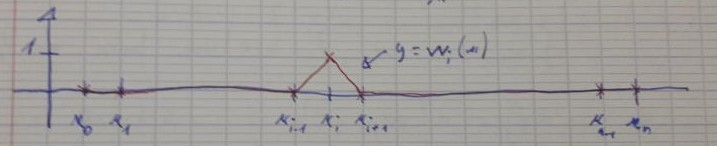
\includegraphics[scale=0.5]{finite_element.png}

  \begin{equation*}
    w_k(t) = 
    \left\{
    \begin{array}{ll}
      \frac{t - t_{k-1}}{t_k - t_{k-1}} & si \quad t \in [t_{k-1},
        t_k] \\
      \frac{t - t_{k+1}}{t_k - t_{k+1}} & si \quad t \in [t_k,
        t_{k+1}] \\
      0 & si \quad t \notin [t_{k-1}, t_{k+1}]
    \end{array}
    \right.
  \end{equation*}

  Si la subdivision est uniforme on a :

  \begin{equation*}
    w_k(t) = 
    \left\{
    \begin{array}{ll}
      \frac{t - t_{k-1}}{h} & si \quad t \in [t_{k-1},
        t_k] \\
      - \frac{t - t_{k-1}}{h} & si \quad t \in [t_k,
        t_{k+1}] \\
      0 & sinon
    \end{array}
    \right.
  \end{equation*}

  $w_k$ est dérivable sur $[a, b]$ donc :

  \begin{equation*}
    w_k'(t) = 
    \left\{
    \begin{array}{ll}
      \frac{1}{h} & si \quad t \in ]t_{k-1},
        t_k[ \\
      - \frac{1}{h} & si \quad t \in ]t_k,
        t_{k+1}[ \\
      0 & sinon
    \end{array}
    \right.
  \end{equation*}

  donc,

  \begin{equation*}
    w_k'(t) = 
    \left\{
    \begin{array}{ll}
      \frac{1}{h} & si \quad t \in ]t_{k-1},
        t_k[ \\
      - \frac{1}{h} & si \quad t \in ]t_k,
        t_{k+1}[ \\
      0 & sinon
    \end{array}
    \right.
  \end{equation*}


\item

\item
  Lorque $|i - j| > 1$, $a(i, j) = 0$. A est une matrice tridiagonale.

\item

\item
  

\end{enumerate}

\section*{Exercice 7}

\section*{Exercice 8}

\newpage

\section*{Annexe}

\textbf{BOUTON NICOLAS}

\lstinputlisting{src/exo1.sci}

\newpage

\lstinputlisting{src/exo2.sci}

\newpage

\lstinputlisting{src/exo3.sci}

\newpage

\lstinputlisting{src/exo4.sci}

\newpage

\lstinputlisting{src/exo5.sci}

\newpage

\lstinputlisting{src/exo6.sci}


\end{document}
